\chapter{Berry Curvature from Maxwell Fields}
\label{ch:berry-maxwell}

\begin{chapterlead}
Topology entered condensed-matter physics through the Berry phase of
electronic Bloch states. The same mathematics applies to photonic Bloch
modes---but with an important difference: the inner product is defined by
the electromagnetic energy, not by the probability density. This chapter
derives Berry connection, Berry curvature, and Chern numbers directly from
the Maxwell eigenproblem, without passing through a tight-binding analogy.
The result is a Maxwell-first topological photonics that connects the
band structure of Chapter~\ref{ch:periodicity} to the existence of
topologically protected edge states.
\end{chapterlead}


%% ================================================================
\section{Why the inner product matters}
\label{sec:inner-product-matters}

Before computing the Berry phase, we must settle a question that has no
analogue in electronic topological insulators: \emph{which inner product
defines the Berry connection?}

In quantum mechanics, the choice is unambiguous: the standard
$L^2$ inner product $\langle\psi|\phi\rangle = \int\psi^*\phi\;\dd^3r$.
In photonics, the natural inner product comes from the electromagnetic
energy density. For nondispersive Hermitian media, the $\EE$-field
formulation uses the weighted product
\begin{equation}
 \langle\mathbf{u}|\mathbf{v}\rangle_\varepsilon
 = \int_{\Omega_{\mathrm{uc}}}
 \epsr(\rr)\,\mathbf{u}^*(\rr)\cdot\mathbf{v}(\rr)\;\dd^d r,
 \label{eq:eps-inner}
\end{equation}
while for the $\HH$-field formulation with $\mur=1$ it is the unweighted
form
\begin{equation}
 \langle\mathbf{u}|\mathbf{v}\rangle
 = \int_{\Omega_{\mathrm{uc}}}
 \mathbf{u}^*(\rr)\cdot\mathbf{v}(\rr)\;\dd^d r.
 \label{eq:h-inner}
\end{equation}
The $\HH$-field formulation leads to the Hermitian eigenoperator
$\hat{\Theta}_H = \curl\bigl(\epsr^{-1}\curl\,\cdot\,\bigr)$ whose
eigenstates are automatically orthogonal in~\eqref{eq:h-inner}. The
$\EE$-field formulation leads to a generalized eigenproblem
$\curl(\mur^{-1}\curl\EE) = (\omega^2/c^2)\epsr\EE$ whose eigenstates
are orthogonal in the $\epsr$-weighted product~\eqref{eq:eps-inner}.

Both formulations give the same Berry curvature and Chern numbers when
$\epsr$ is Hermitian (real for scalar, Hermitian for tensor), because
the eigenstates are related by a gauge transformation. However, the
$\epsr$-weighted inner product is the physically correct one for
perturbation theory, for normalization of mode amplitudes, and for the
construction of Wannier functions~\cite{paz2019tutorial}. In dispersive
but lossless media, $\epsr$ is replaced by the Brillouin energy weight
discussed in Chapter~\ref{ch:loss-gain-dispersion}.

\begin{remark}
In non-Hermitian systems (complex $\epsr$), the two formulations lead
to different Berry connections because the $\epsr$-weighted inner
product is no longer positive definite. The resolution requires the
biorthogonal Berry connection of Section~\ref{sec:nh-berry-preview} and
Chapter~\ref{ch:complex-bands}.
\end{remark}


%% ================================================================
\section{Geometric phase for photonic Bloch states}
\label{sec:berry-photonic}

Recall from Chapter~\ref{ch:periodicity} that the Bloch eigenmodes of a
periodic photonic crystal satisfy the unit-cell eigenproblem
$\Mop_\kk\,\mathbf{u}_{n\kk} = (\omega_n(\kk)^2/c^2)\,\mathbf{u}_{n\kk}$,
with $\mathbf{u}_{n\kk}(\rr)$ periodic on $\Omega_{\mathrm{uc}}$.
As $\kk$ varies over the Brillouin zone, $\mathbf{u}_{n\kk}$ traces a
path in the Hilbert space of periodic vector fields. The geometric phase
accumulated along this path is the photonic Berry phase.

\subsection{Berry connection}
\label{ssec:berry-connection}

The \emph{Berry connection} for band $n$ is the one-form on the
Brillouin zone defined by~\cite{paz2019tutorial}
\begin{equation}
 \Acal_{n,\alpha}(\kk) = i\,
 \frac{\langle\mathbf{u}_{n\kk}|\partial_{k_\alpha}|\mathbf{u}_{n\kk}\rangle_\varepsilon}
 {\langle\mathbf{u}_{n\kk}|\mathbf{u}_{n\kk}\rangle_\varepsilon},
 \label{eq:berry-connection}
\end{equation}
where $\alpha = x, y$ labels the components of $\kk$ and the inner
product is the $\epsr$-weighted form~\eqref{eq:eps-inner}. When the
modes are normalized to
$\langle\mathbf{u}_{n\kk}|\mathbf{u}_{n\kk}\rangle_\varepsilon = 1$,
the denominator drops out.

The Berry connection is \emph{gauge-dependent}: under a gauge
transformation $|\mathbf{u}_{n\kk}\rangle \to e^{i\phi(\kk)}|\mathbf{u}_{n\kk}\rangle$,
it shifts by $\Acal_{n,\alpha} \to \Acal_{n,\alpha} - \partial_{k_\alpha}\phi$. Physical
observables must therefore depend on gauge-invariant combinations.

\subsection{Berry curvature}
\label{ssec:berry-curvature}

The \emph{Berry curvature} is the gauge-invariant curl of the Berry
connection. In two dimensions ($\kk = (k_x,k_y)$), it is a
pseudoscalar:
\begin{equation}
 \Fcal_n(\kk) = \pdv{\Acal_{n,y}}{k_x} - \pdv{\Acal_{n,x}}{k_y}.
 \label{eq:berry-curvature-2d}
\end{equation}
An equivalent expression that does not require differentiating the
Berry connection directly is the Kubo-like formula:
\begin{equation}
 \Fcal_n(\kk) = -2\sum_{m\neq n}
 \frac{\Im\bigl[
 \langle\mathbf{u}_{n\kk}|\partial_{k_x}\Mop_\kk|\mathbf{u}_{m\kk}\rangle_\varepsilon
 \;\langle\mathbf{u}_{m\kk}|\partial_{k_y}\Mop_\kk|\mathbf{u}_{n\kk}\rangle_\varepsilon
 \bigr]}
 {[\omega_n^2(\kk) - \omega_m^2(\kk)]^2}.
 \label{eq:berry-curvature-kubo}
\end{equation}
This formula shows that the Berry curvature is large when two bands
are nearly degenerate ($\omega_n \approx \omega_m$)---the curvature is
concentrated near avoided crossings and symmetry points.

\subsection{Physical interpretation}
\label{ssec:berry-physics}

The Berry curvature has a direct physical interpretation: it is the
``magnetic field'' in momentum space that deflects wave packets
transversely. For a photonic wave packet centered at $\kk$ in band $n$,
the semiclassical equations of motion include an anomalous velocity
\begin{equation}
 \dot{\rr}_{\perp} = -\dot{\kk}\times\hat{z}\,\Fcal_n(\kk),
 \label{eq:anomalous-velocity}
\end{equation}
which deflects the wave packet perpendicular to both the applied force
$\dot{\kk}$ and the direction of propagation. This is the photonic
analogue of the anomalous Hall effect in electronic systems~\cite{skirlo2015experimental,wu2015scheme,noh2017observation,chen2018valley,gao2017topologically,kang2018pseudo,he2019silicon,tan2021scheme,ma2017scattering,hui2021photonic}. When the
Berry curvature has a definite sign across the Brillouin zone, the
deflection is systematic and produces a net transverse photon current---the
photonic Hall effect.

\paragraph{Example: Berry curvature near a Dirac point.}
Consider a triangular-lattice photonic crystal of dielectric rods
($\varepsilon = 12$, radius $r = 0.2a$) in air. The TM band structure
has a Dirac point at the $K$ corner of the Brillouin zone between the
second and third bands. Near this degeneracy, the two-band effective
Hamiltonian takes the massive Dirac form
\begin{equation}
 H_{\mathrm{eff}}(\delta\kk) = v_D(\delta k_x\,\sigma_x + \delta k_y\,\sigma_y)
 + \tfrac{1}{2}m\,\sigma_z,
 \label{eq:dirac-berry-eff}
\end{equation}
where $v_D$ is the group velocity at the Dirac point, $m$ is the gap
opened by a perturbation (e.g.\ by breaking $C_3$ inversion symmetry or
applying a magneto-optical field), and $\delta\kk = \kk - \kk_K$. The
Berry curvature of the lower band is
\begin{equation}
 \Fcal(\delta\kk) = -\frac{m\,v_D^2}
 {4(v_D^2|\delta\kk|^2 + m^2/4)^{3/2}}.
 \label{eq:dirac-berry-curvature}
\end{equation}
This is sharply peaked at $\delta\kk = 0$: the Berry curvature is
concentrated within a momentum radius $\sim |m|/(2v_D)$ of the Dirac
point. The integral over a single valley gives a half-integer valley
contribution whose sign is set by both the Dirac mass and the chirality
of that valley. For a Haldane-like magneto-optical perturbation, the
mass and valley chirality combine so that the two valley contributions
add rather than cancel, giving a nonzero total Chern number. Reversing
the bias field reverses the sign of the total Chern number.

This example illustrates a key principle: the Chern number is determined
by the \emph{local} Berry curvature near band degeneracies. The rest of
the Brillouin zone contributes negligibly. This is why photonic
topological transitions are controlled by gap closings and reopenings
at high-symmetry points.


%% ================================================================
\section{Chern number}
\label{sec:chern}

The integral of the Berry curvature over the entire Brillouin zone is
quantized:
\begin{equation}
 \boxed{
 \Chern_n = \frac{1}{2\pi}\int_{\BZ}\Fcal_n(\kk)\;\dd^2 k
 \;\in\;\mathbb{Z}.
 }
 \label{eq:chern}
\end{equation}
This integer is the \emph{Chern number} of the $n$-th band. It is a
topological invariant: it cannot change under smooth deformations of the
band structure that do not close the gap to an adjacent
band~\cite{paz2019tutorial}.

\subsection{Quantization proof sketch}
\label{ssec:chern-proof}

The quantization of the Chern number follows from a general result in
differential geometry: the integral of a curvature two-form over a
closed manifold (here, the Brillouin zone torus $T^2$) is $2\pi$ times
an integer. Physically, the argument proceeds as follows:
\begin{enumerate}
 \item Divide the BZ into patches on each of which a smooth gauge for
 $|\mathbf{u}_{n\kk}\rangle$ can be chosen.
 \item On the overlap between two patches, the gauge transformation
 $e^{i\phi(\kk)}$ is single-valued and smooth.
 \item The Berry curvature integral equals the total winding of the
 gauge transformation around the patch boundaries, which is an
 integer by the single-valuedness of $e^{i\phi}$.
\end{enumerate}

\subsection{Time-reversal symmetry}
\label{ssec:time-reversal-berry}

When the photonic crystal preserves time-reversal symmetry
($\epsr(\rr)$ real and scalar), the Berry curvature satisfies
$\Fcal_n(\kk) = -\Fcal_n(-\kk)$, and the Chern number vanishes:
$\Chern_n = 0$. Nonzero Chern numbers require breaking time-reversal
symmetry, for example with a magneto-optical material~\cite{he2016photonic,chen2023berry,yang2018realization,khanikaev2016three,horiuchi2013photonic,slobozhanyuk2015observation,gao2016probing}
($\epsr$ tensor with off-diagonal imaginary components).

The proof is straightforward: time reversal maps $\kk \to -\kk$ and
complex-conjugates the eigenvectors. The Berry curvature, being the
imaginary part of an overlap integral, picks up a sign from the
conjugation and another sign from the reversal of $\kk$, giving
$\Fcal_n(-\kk) = -\Fcal_n(\kk)$.

\subsection{Valley Chern number}
\label{ssec:valley-chern}

Even when $\Chern_n = 0$ globally, the Berry curvature may be
concentrated near specific high-symmetry points (valleys) in the
Brillouin zone. The \emph{valley Chern number}
\begin{equation}
 \Chern_n^{(v)} = \frac{1}{2\pi}
 \int_{\text{valley}}\Fcal_n(\kk)\;\dd^2 k
 \label{eq:valley-chern}
\end{equation}
can be half-integer and is approximately quantized when the valley
is well separated from other regions of nonzero curvature. Valley
Chern numbers underlie the photonic valley Hall effect, in which light
propagates along domain walls between regions with opposite valley
orientations.

%% ================================================================
\section{Photonic Chern insulators}
\label{sec:photonic-chern}

\subsection{Magneto-optical photonic crystals}
\label{ssec:magneto-optical}

The canonical platform for nonzero photonic Chern numbers~\cite{haldane2008possible,wang2009observation,hafezi2013imaging,haldane2008reflection} is a
two-dimensional photonic crystal made from magneto-optical material.
Under a static magnetic field $\BB_0 = B_0\hat{z}$, a ferrite or
yttrium iron garnet (YIG) develops an antisymmetric permittivity tensor:
\begin{equation}
 \boldsymbol{\varepsilon} = \begin{pmatrix}
 \varepsilon_{xx} & i\varepsilon_g & 0 \\
 -i\varepsilon_g & \varepsilon_{xx} & 0 \\
 0 & 0 & \varepsilon_{zz}
 \end{pmatrix},
 \label{eq:magneto-optical-eps}
\end{equation}
where $\varepsilon_g \propto B_0$ is the gyromagnetic coupling. This
tensor is Hermitian ($\boldsymbol{\varepsilon}^\dagger =
\boldsymbol{\varepsilon}$) but not symmetric
($\boldsymbol{\varepsilon}^\transpose \neq \boldsymbol{\varepsilon}$):
the system is lossless but breaks time-reversal symmetry.

The breaking of time-reversal symmetry lifts the $\Fcal_n(\kk) =
-\Fcal_n(-\kk)$ constraint, allowing nonzero Chern numbers. For a
triangular-lattice photonic crystal of YIG rods in air, with parameters
$\varepsilon_{xx} = 15$, $\varepsilon_g = 12.4$ (at microwave
frequencies near $4.28\;\mathrm{GHz}$), numerical calculations give
$\Chern = \pm 1$ for the lowest-frequency TM gap.

\paragraph{Worked Chern-number calculation.}
To make the calculation concrete, consider a square lattice of YIG
cylinders (radius $r = 0.11a$) in air with the tensor
permittivity~\eqref{eq:magneto-optical-eps} and parameters
$\varepsilon_{xx} = 15$, $\varepsilon_g = 12.4$. The TM modes
($E_z$ polarisation) satisfy a scalar eigenproblem whose $\kk$-dependent
operator is $\Mop_\kk = -(\nabla + i\kk)\times(\boldsymbol{\varepsilon}^{-1}(\nabla + i\kk)\times)$.
The inverse permittivity tensor couples $E_z$ to the in-plane magnetic
field components, breaking the degeneracy between clockwise and
counter-clockwise circulating modes at the $\Gamma$ and $M$ points.

Numerical diagonalisation on a $201\times201$ $\kk$-grid using the FHS
algorithm~\eqref{eq:fhs} yields $\Chern_1 = +1$ for the lowest band
(below the first gap) and $\Chern_2 = -2$ for the second band, giving a
gap Chern number $\Chern_{\mathrm{gap}} = +1$ for the first gap. The
Berry curvature is concentrated at the $M$ point, where the gap is
smallest ($\Delta\omega/\omega_0 \approx 0.08$), confirming that the
topological invariant is controlled by the near-degenerate region. When
the magnetic field is reversed ($\varepsilon_g \to -\varepsilon_g$), all
Chern numbers change sign: $\Chern_{\mathrm{gap}} = -1$, so the edge
state propagation direction reverses.

\subsection{Photonic anomalous Hall effect}
\label{ssec:photonic-hall}

A photonic crystal with $\Chern \neq 0$ is a \emph{photonic Chern
insulator}. The bulk-boundary correspondence
(Section~\ref{sec:bbc-hermitian}) guarantees one-way edge states at
every interface with a topologically distinct region (including vacuum,
which has $\Chern = 0$).

These chiral edge modes propagate in one direction only and are immune
to backscattering from fabrication defects, sharp bends, or surface
roughness---as long as the bulk gap remains open. This is the photonic
anomalous Hall effect: electromagnetic energy flows in one direction
along the edge, with the direction determined by the sign of the Chern
number and hence by the direction of the applied magnetic field.

\begin{figure}[t]
 \centering
 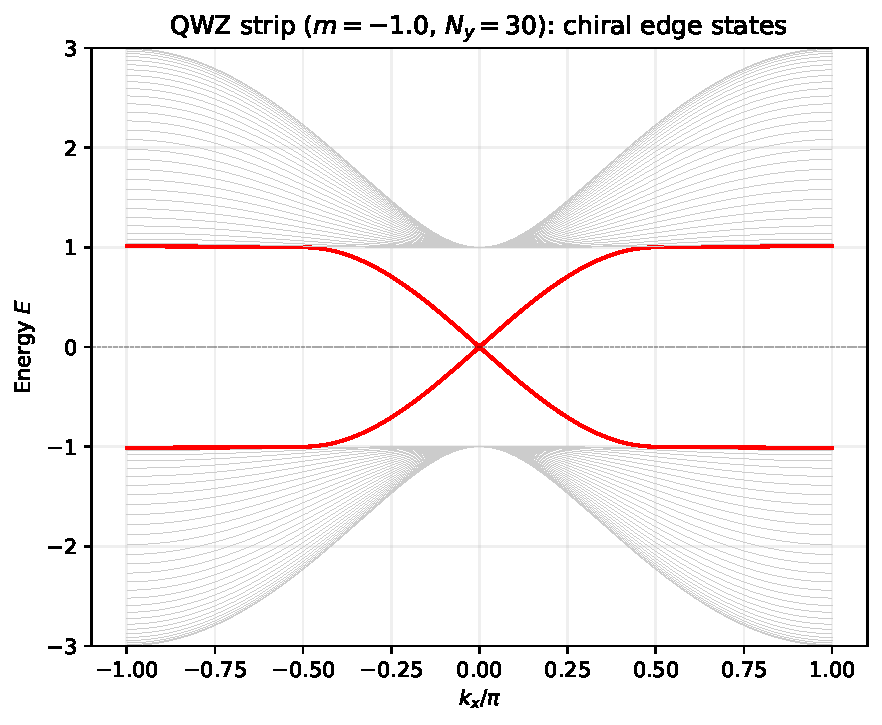
\includegraphics[width=0.6\linewidth]{figures/fig_f11_chiral_edge.pdf}
 \caption{Computed band structure of a QWZ strip ($m = -1$, $N_y = 30$).
 The 60 bulk bands (grey) form a gapped spectrum with Chern number
 $\Chern = 1$. The red branches are edge-localized modes on the two
 opposite strip boundaries; each boundary supports one chiral channel,
 with opposite group velocities on opposite edges. The branches connect
 the lower and upper bulk bands across the gap, illustrating the
 bulk--boundary correspondence.}
 \label{fig:chiral-edge-strip}
\end{figure}

\paragraph{Experimental observation.}
The photonic anomalous Hall effect was first demonstrated experimentally
by Wang et al.\ (2009) using a two-dimensional photonic crystal of YIG
rods at microwave frequencies. The experiment confirmed three
predictions of the topological theory:
\begin{enumerate}
 \item One-way edge propagation with suppressed backscattering even
 around sharp $90^\circ$ bends and metallic obstacles.
 \item The number of edge modes matches the predicted Chern number
 difference across the interface.
 \item Reversal of the external magnetic field reverses the
 propagation direction, confirming the topological origin.
\end{enumerate}
The key quantitative figure of merit is the ratio of forward to backward
transmission: in the experiment, this exceeded $50\;\mathrm{dB}$ across
the topological gap, comparable to commercial microwave isolators but
achieved without any Faraday-rotation element.

\subsection{Limitations}
\label{ssec:chern-limitations}

The magneto-optical approach has practical limitations:
\begin{itemize}
 \item The gyromagnetic effect is weak at optical frequencies, so
 large Chern gaps require strong magnetic fields or resonant
 enhancement.
 \item The materials are typically lossy, introducing non-Hermiticity
 that complicates the topological classification.
 \item The platform is most practical at microwave and millimeter-wave
 frequencies, where ferrites have large gyromagnetic responses.
\end{itemize}
Alternative approaches---Floquet modulation, coupled-ring lattices, and
synthetic gauge fields---can produce effective Chern insulators at
optical frequencies without magnetic materials.

\paragraph{Floquet photonic Chern insulators.}
An alternative route to nonzero Chern numbers at optical frequencies uses
time-periodic modulation of the refractive index~\cite{rechtsman2013photonic,ozawa2018topological}. The central idea is
that a periodically driven system has a \emph{Floquet Hamiltonian}
$H_F$ whose eigenvalues are quasi-energies $\varepsilon_n$ defined
modulo the driving frequency $\Omega$. Even if the instantaneous
Hamiltonian preserves time-reversal symmetry at every instant, the
stroboscopic evolution operator $U(T) = \mathcal{T}\exp(-i\int_0^T
H(t)\,\dd t)$ can break effective time-reversal symmetry, opening
topological gaps with nonzero Chern numbers.

The simplest photonic implementation uses a two-dimensional lattice
of coupled waveguides or ring resonators with periodically modulated
link phases. The paraxial propagation equation along the waveguide
axis $z$ plays the role of the Schr\"odinger equation:
\begin{equation}
 i\partial_z \psi(x,y,z) = H(z)\,\psi(x,y,z),
 \label{eq:paraxial-floquet}
\end{equation}
where $z$ replaces time and the lattice potential $H(z)$ is periodic
with period $Z$ (the helix pitch or modulation period). The Floquet
operator $U(Z) = \mathcal{T}\exp(-i\int_0^Z H(z')\,\dd z')$ defines
the effective Hamiltonian $H_F = (i/Z)\ln U(Z)$, and its Bloch bands
carry well-defined Chern numbers computed from the Berry curvature of
the Floquet eigenstates.

In coupled-ring-resonator lattices~\cite{hafezi2013imaging}, the link phases between
rings are engineered to simulate an effective magnetic vector potential
$\mathbf{A}_{\mathrm{eff}}$, producing Floquet bands with nonzero
Chern numbers. The key advantage is that no magnetic material is
required: time-reversal symmetry is broken by the modulation itself.
Chiral edge states have been observed experimentally in
silicon-photonic ring-resonator networks at telecom wavelengths,
demonstrating topological protection at optical frequencies with
forward-to-backward transmission contrast exceeding $10\;\mathrm{dB}$.

\paragraph{Non-Hermitian complications in Floquet systems.}
The main limitation of Floquet topological photonics is that
driven systems are inherently open: they exchange energy with the
driving field and with the environment. Material loss, radiation
leakage, and gain saturation all make the effective Floquet Hamiltonian
non-Hermitian. The quasi-energy bands become complex, and the Chern
number must be replaced by its biorthogonal generalization
(Chapter~\ref{ch:complex-bands}). Furthermore, Floquet systems can
exhibit parametric instability when the driving frequency is resonant
with inter-band transitions, leading to exponential growth of certain
modes---a Floquet-specific mechanism of non-Hermiticity that has no
static analogue. These complications connect the Floquet approach
directly to the non-Hermitian Berry connection of
Section~\ref{sec:nh-berry-preview} and the open problems of
Chapter~\ref{ch:open-problems}.


%% ================================================================
\section{Wilson loop and $\mathbb{Z}_2$ invariants}
\label{sec:wilson-loop}

For systems with time-reversal symmetry where the Chern number vanishes,
topological information is encoded in the \emph{Wilson loop}
operator~\cite{paz2019tutorial}:
\begin{equation}
 W(\ell) = \mathcal{P}\exp\!\left[-i\oint_\ell
 \mathbf{A}(\kk)\cdot\dd\kk\right],
 \label{eq:wilson-loop}
\end{equation}
where $\mathbf{A}$ is the non-Abelian Berry connection matrix for a group
of $N$ bands, $(\mathbf{A})_{mn} = i\langle\mathbf{u}_{m\kk}|\nabla_\kk|\mathbf{u}_{n\kk}\rangle_\varepsilon$,
and $\mathcal{P}$ denotes path ordering.

The eigenvalues of $W(\ell)$---the Wannier center flow---reveal the
topological phase:
\begin{itemize}
 \item \textbf{Trivial phase:} Wannier centers are constant (do not
 wind) as a function of the free momentum parameter.
 \item \textbf{$\mathbb{Z}_2$ topological phase:} Wannier centers wind
 by $\pm 2\pi$ across the Brillouin zone, corresponding to
 delocalized Wannier functions.
 \item \textbf{Obstructed atomic limit:} Wannier centers are pinned at
 non-trivial positions but do not wind.
 \item \textbf{Fragile topology:} Wannier centers wind with opposite
 slopes, and the topology can be unwound by adding trivial bands.
\end{itemize}


%% ================================================================
\section{Numerical computation}
\label{sec:berry-numerical}

\subsection{Discretized Berry curvature}
\label{ssec:discretized}

On a discrete grid of $\kk$-points in the Brillouin zone, the Berry
curvature is computed from the gauge-invariant lattice formula of
Fukui, Hatsugai, and Suzuki (FHS):
\begin{equation}
 \Fcal_n(\kk) \approx -\Im\ln\!\bigl[
 U_1(\kk)\,U_2(\kk+\delta k_1\hat{e}_1)\,
 U_1^*(\kk+\delta k_2\hat{e}_2)\,U_2^*(\kk)
 \bigr],
 \label{eq:fhs}
\end{equation}
where
\begin{equation}
 U_\alpha(\kk)=
 \frac{\langle\mathbf{u}_{n\kk}|
 \mathbf{u}_{n,\kk+\delta k_\alpha\hat{e}_\alpha}\rangle_\varepsilon}
 {|\langle\mathbf{u}_{n\kk}|
 \mathbf{u}_{n,\kk+\delta k_\alpha\hat{e}_\alpha}\rangle_\varepsilon|}
 \label{eq:fhs-link}
\end{equation}
is the phase-only link variable between adjacent $\kk$-points in
direction $\alpha$.
This formula is manifestly gauge-invariant and numerically robust: it
does not require a smooth global gauge choice~\cite{paz2019tutorial}.

\begin{figure}[t]
 \centering
 
\includegraphics[width=0.95\textwidth]{fig_f11_berry_curvature_chern.pdf}
 \caption{Gauge-invariant Berry-curvature computation with the FHS link-variable algorithm. The plotted model is a two-band lattice Dirac model used as a pedagogical proxy for Maxwell Bloch bands: in a photonic calculation, the spinor overlaps are replaced by energy-inner-product overlaps of Maxwell modes. The left panel shows the analytic Berry-curvature density $\mathcal{F}_{xy}(\kk)$ for the QWZ model at $m=-1$, using the sign convention whose Brillouin-zone integral gives $C=1$. The right panel shows the FHS quantization residual $|C_N-1|$ for selected $N\times N$ grids, demonstrating machine-precision integer quantization.}
 \label{fig:berry-curvature-chern}
\end{figure}

\subsection{Practical considerations}
\label{ssec:numerical-practical}

Several practical issues arise when computing the photonic Berry
curvature numerically:
\begin{enumerate}
 \item \textbf{Band labeling:} at near-degenerate $\kk$-points, the
 eigensolver may swap band labels. The link-variable approach
 mitigates this because the overlap $U_\alpha$ automatically tracks
 the smooth band, but the grid spacing $\delta k$ must be small
 enough that the overlap is close to unity.
 \item \textbf{Grid resolution:} the Berry curvature is typically
 peaked near degeneracies and high-symmetry points. An adaptive
 grid or a finer mesh near these features improves accuracy without
 excessive computational cost.
 \item \textbf{Multi-band Chern number:} when two or more bands are
 separated from others by a common gap, the total Chern number of
 the group is computed from the non-Abelian Berry curvature
 $\Fcal_{mn}$ using
 $\Chern = (2\pi)^{-1}\int_{\BZ}\tr\Fcal\;\dd^2 k$.
 \item \textbf{Gauge smoothing:} for Wilson-loop calculations, a
 smooth gauge across one direction of the BZ is needed. The
 standard method is to fix the gauge on a reference line and
 parallel-transport it across the BZ using the SVD of the overlap
 matrix.
\end{enumerate}

\subsection{Chern number from integration}
\label{ssec:chern-numerical}

For the FHS formula, $\Fcal_n(\kk)$ is already the Berry flux through a
plaquette, so the Chern number is
\begin{equation}
 \Chern_n = \frac{1}{2\pi}\sum_{\text{plaquettes}}\Fcal_n(\kk).
 \label{eq:fhs-chern-sum}
\end{equation}
No additional factor of $\Delta k_x\,\Delta k_y$ is included. The result
is automatically an integer up to numerical precision because the
lattice formula captures the correct topology.


%% ================================================================
\section{Bulk-boundary correspondence}
\label{sec:bbc-hermitian}

The most striking physical consequence of a nonzero Chern number is the
existence of topologically protected edge states. The
\emph{bulk-boundary correspondence} states that the number of chiral edge
modes at an interface between two insulators is equal to the difference of
their gap Chern numbers:
\begin{equation}
 N_{\mathrm{edge}} = \Chern_{\mathrm{gap}}^{(\mathrm{left})}
 - \Chern_{\mathrm{gap}}^{(\mathrm{right})}.
 \label{eq:bbc}
\end{equation}
These edge states propagate in one direction only and are robust against
backscattering from disorder or defects: their existence is guaranteed by
topology, not by fine-tuned material parameters.

\subsection{Edge dispersion}
\label{ssec:edge-dispersion}

The chiral edge states have a dispersion relation $\omega(k_\parallel)$
that crosses the bulk gap. The group velocity $v_g = \dd\omega/\dd
k_\parallel$ has a definite sign (positive or negative) determined by the
Chern number. The edge modes connect the bulk bands above and below the
gap, interpolating smoothly between the valence and conduction bands.
The number of crossings equals $|\Chern|$, providing a graphical check
of the bulk-boundary correspondence.

\subsection{Robustness}
\label{ssec:edge-robustness}

In photonic Chern insulators (realized with magneto-optical materials),
the chiral edge states provide one-way waveguides for light---immune to
backscattering from fabrication imperfections, sharp bends, or surface
roughness. The robustness has a simple topological explanation: a
backscattered wave would need to reverse its direction, which requires
coupling to a counter-propagating edge mode. But only one direction of
propagation is available at each edge (there is no counter-propagating
channel), so backscattering is forbidden by topology.

This topological protection is exact in the limit of an infinite bulk
gap and degrades gradually as the gap closes. In practice, the
backscattering suppression is exponential in the ratio of the gap width
to the defect strength.

\begin{takeaway}[Hermitian bulk-boundary correspondence]
In Hermitian photonic crystals, the Chern number computed from the
Maxwell Bloch states determines the number of topologically protected
one-way edge channels. This correspondence is exact and robust: it
survives disorder, deformation, and any perturbation that does not close
the bulk gap. In non-Hermitian systems, this correspondence can fail;
the skin effect and non-Bloch bulk-boundary correspondence are the
subject of Chapters~\ref{ch:skin-effect} and~\ref{ch:bbc-rebuilt}.
\end{takeaway}


%% ================================================================
\section{Preview: non-Hermitian modifications}
\label{sec:nh-berry-preview}

The Berry curvature and Chern number derived above assumed a Hermitian
inner product and real eigenfrequencies. When non-Hermiticity is
introduced:
\begin{enumerate}
 \item The eigenfrequencies $\omega_n(\kk)$ become complex, and ``band
 gaps'' must be redefined in the complex frequency plane
 (Chapter~\ref{ch:complex-bands}).
 \item The left and right eigenvectors differ, and the Berry
 connection must be generalized to a \emph{biorthogonal} form:
 \begin{equation}
 \Acal_n^{\mathrm{bi}} = i\,
 \frac{\langle\mathbf{u}_n^{\mathrm{L}}|\nabla_\kk|\mathbf{u}_n^{\mathrm{R}}\rangle}
 {\langle\mathbf{u}_n^{\mathrm{L}}|\mathbf{u}_n^{\mathrm{R}}\rangle}.
 \label{eq:biorthogonal-berry-preview}
 \end{equation}
 The appropriate bilinear pairing depends on the Maxwell formulation
 and material dispersion; the key point is that the left mode supplies
 the dual vector. The biorthogonal Berry connection is generally
 complex-valued, and its imaginary part tracks changes in the
 left--right normalization rather than an ordinary geometric phase.
 \item New topological invariants---spectral winding numbers and
 point-gap invariants---appear that have no Hermitian analogue
 (Chapter~\ref{ch:point-gap}).
 \item The bulk-boundary correspondence can fail: the bulk Chern number
 may predict edge states that are absent, or miss states that are
 present, due to the non-Hermitian skin effect
 (Chapter~\ref{ch:skin-effect}).
\end{enumerate}

Part~IV of this book develops each of these modifications, building on
the Hermitian topological foundation established in this chapter.

\subsection{From Hermitian to biorthogonal: what changes physically}
\label{ssec:biorthogonal-physical}

The transition from Hermitian to non-Hermitian Berry curvature is not
merely a mathematical generalization; it changes the physical content
of the topological invariants.

In the Hermitian case, the Berry curvature~\eqref{eq:berry-curvature-2d}
is real-valued and determines the transverse deflection of wave packets
via~\eqref{eq:anomalous-velocity}. The Chern number counts chiral edge
modes. Both are observable through intensity measurements.

In the non-Hermitian case, the biorthogonal Berry
connection~\eqref{eq:biorthogonal-berry-preview} is generically
complex. Its real part generalizes the Hermitian Berry phase and can
govern geometric interference effects. Its imaginary part measures
geometric amplification or attenuation associated with changes in the
left--right normalization, and is closely tied to eigenvector
non-orthogonality. Near an exceptional point the biorthogonal eigenbasis
becomes singular, and encircling the defect produces the characteristic
half-integer vorticity discussed in later chapters.

The biorthogonal Chern number
\begin{equation}
 \Chern_n^{\mathrm{bi}} = \frac{1}{2\pi}\int_{\BZ}
 \Fcal_n^{\mathrm{bi}}(\kk)\;\dd^2 k
 \label{eq:biorthogonal-chern}
\end{equation}
remains integer-valued for an isolated band over the Brillouin-zone
torus, provided a smooth biorthogonal basis exists and no exceptional
degeneracy pierces the integration surface. When the relevant gap is a
point gap rather than a line gap, the natural invariant is instead a
spectral winding number of the complex band or Bloch Hamiltonian. That
shift from Chern edge-mode counting to point-gap winding and skin-effect
physics is one of the central themes of Part~IV.
